\documentclass[parskip=full]{scrartcl}
\usepackage[utf8]{inputenc} % use utf8 file encoding for TeX sources
\usepackage[T1]{fontenc}    % avoid garbled Unicode text in pdf
\usepackage[german]{babel}  % german hyphenation, quotes, etc
\usepackage{hyperref}       % detailed hyperlink/pdf configuration
\hypersetup{                % ‘texdoc hyperref‘ for options
pdftitle={SWT1: Lastenheftvorlage},%
bookmarks=true,%
}
\usepackage{graphicx}       % provides commands for including figures
\usepackage{csquotes}       % provides \enquote{} macro for "quotes"
\usepackage[nonumberlist]{glossaries}     % provides glossary commands
\usepackage{enumitem}

\makeglossaries

\title{iMage Online Verkaufplatform}
\author{Ari Nubar Boyacıoğlu, 1960732}

\begin{document}

\maketitle

%
% % Hier beginnt die Gliederung des Lastenhefts
%
\section{Zielbestimmung}
Für den Verkauf des Produkts iMage soll ein Onlinesystem erstellt werden. 

\section{Produkteinsatz}

Das Onlinesystem dient zu den \glspl{Kunde} und den \glspl{Mitarbeiter}n der Vertriebsabteilung. In das Onlinesystem sollen das Programm iMage und seine Plug-ins mit den Preisen angeboten werden.
Die Kunden sollen das Programm und gewünschte Plug-ins kaufen können. Die Mitarbeiter der Vertriebsabteilung sollen die Preise der Produkte anbieten, ändern und Sonderangebote erstellen können.
Das Produkt dient zur Kunden- und Seminarverwaltung der Firma Teachware. Außerdem sollen verschiedene Anfragen beantwortet werden können.

Zielgruppe: Kunden der Firma, Mitarbeiter der Vertriebsabteilung.

Plattformen:	
\begin{itemize}[nosep]  
	\item \gls{Computer} mit Betriebssystemen Windows, MacOS, Linux.
	\item \gls{Tablett}, \gls{Smartphone} mit Betriebssystemen Android, iOS. 
\end{itemize} 
				
\newpage
\section{Funktionale Anforderungen}
\begin{itemize}[nosep]
\item[FA10] Ersterfassung, Änderung und Löschung von Kundenrechnungen.
\item[FA20] Benachrichtigung der Kunden (Anmeldebestätigung, Abmeldebestätigung, Änderungsmitteilungen, Rechnung, Werbung).
\item[FA30] Ersterfassung, Änderung und Löschung von verkaufenden Produkten.
\item[FA40] Ersterfassung, Änderung und Löschung von Sonderangebote der Produkte.
\item[FA50] Erstellung verschiedener Listen (Produktlisten, Sonderangebotlisten).
\item[FA60] Erstellung eines Warenkorbsystems für die gewählte und bestellte Produkte.
\item[FA70] Erstellung von einem Bewertungssystem für die meist bevorzugten Produkten.
\item[FA80] Integration der Zahlsystemen (z.B PayPal, Visa usw.)
\item[FA90] Vorstellung der Preisesparnis der Sonderangebote gegenüber dem Einzelkauf der Produkte.
\item[FA100] Erstellung \gls{Support-Ticketsystem}s für Lösung eventuellen Kundenproblemen.
\end{itemize}

\section{Produktdaten}
\begin{itemize}[nosep]
\item[PD10] Relevante Daten über Kunden (Adresse, Telefonnummer, E-Post Adresse, bevorzugte Zahlmethode) sind zu speichern.
\item[PD20] Relevante Daten über Produkte (Preis, Sonderangebote, Preisesparnis) sind zu speichern. 
\item[PD30] Bestellt ein Kunde ein Produkt, dann sind entsprechende Bestelldaten zu speichern.
\end{itemize}

\section{Nichtfunktionale Anforderungen}
\begin{itemize}[nosep]
\item[NF10] In /FA10/ kann pro Person eine Rechnung erfasst werden.
\item[NF20] Eine Adresse, ein Telefonnummer und eine e-Mail Adresse sind Voraussetzungen des Erstellen eines Kontos und der Bestellung eines Produkts.
\item[NF30] Es müssen maximal 250.000 Kunden gleichzeitig gedient werden können.
\end{itemize}


\section{Systemmodelle}

\subsection{Szenarien}

\subsubsection{Mitarbeiter/Moderatoren Können:}
\begin{itemize}[nosep]
	\item Neue Produkte mit den Beschreibungen vorstellen.
	\item Die Preise der Produkte erstellen, ändern.
	\item Sonderangebote erstellen, ändern.
	\item Tickets beantworten, schliessen.
	\item Daten/Warenkörbe der Kunden kontrollieren.
	\item Rating-System anschauen.
\end{itemize}
\subsubsection{Kunden Können:}
\begin{itemize}[nosep]
	\item Eine Kundenrechnung erstellen bzw. löschen, die Daten der Rechnung ändern.
	\item Produkte anschauen, in den Warenkorb anlegen.
	\item Die Produkte in dem Warenkorb bestellen.
	\item Sonderangebote vergleichen.
	\item Tickets eröffnen.
	\item Produkte bewerten.
\end{itemize}

\subsection{Anwendungsfälle}
\subsubsection{Seminarorganisation}
\begin{center}
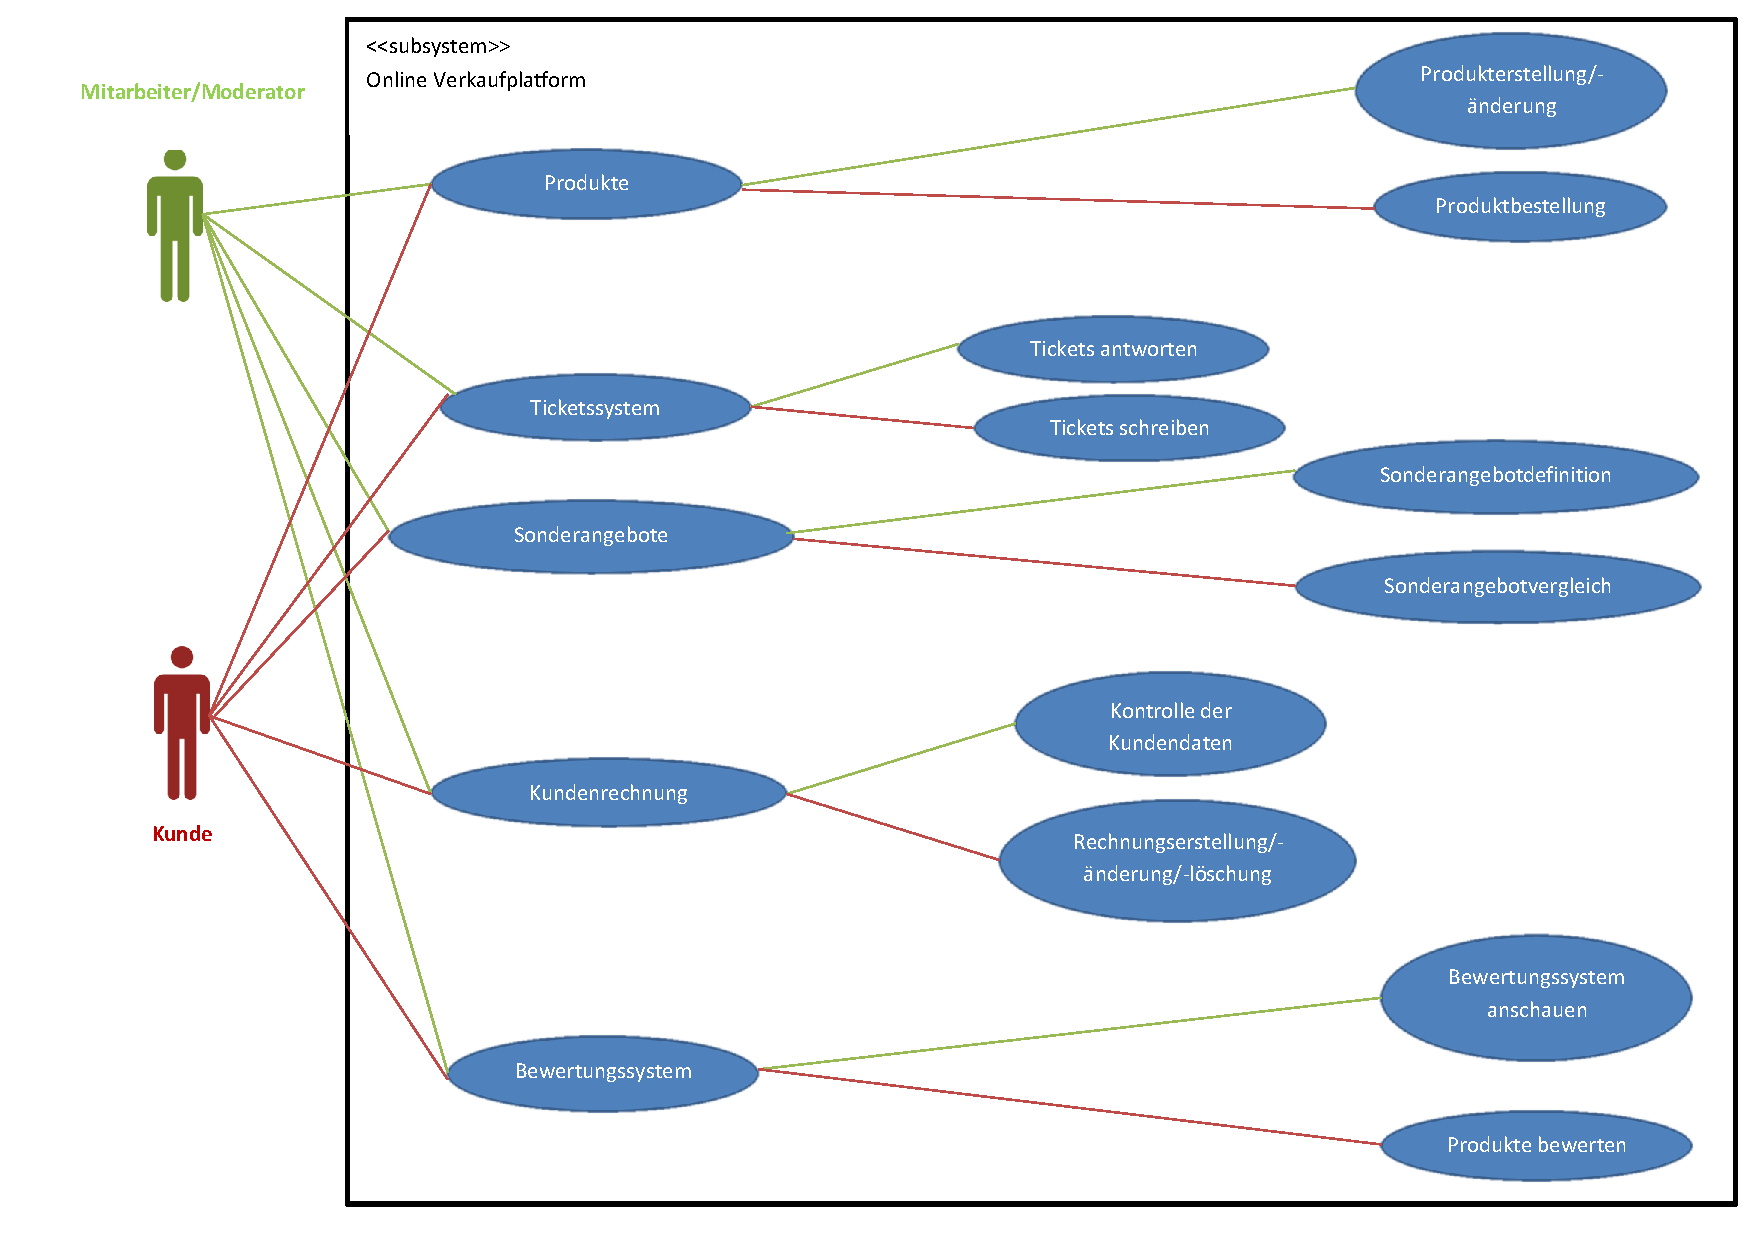
\includegraphics[width=0.9\textwidth]{szenario_onlineverkaufplatform.pdf}
\end{center}

Akteure: Kunde, Mitarbeiter/Moderator.

Anwendungsfälle: 
\begin{enumerate}
	\item Produkte
	\begin{enumerate}
		\item Produkterstellung
		\item Produktänderung
		\item Produktbestellung
	\end{enumerate}
\item Ticketssystem
	\begin{enumerate}
		\item Ticket schreiben
		\item Ticket antworten
	\end{enumerate}
\item Sonderangebote
	\begin{enumerate}
		\item Sonderangebotdefinition
		\item Sonderangebotvergleich
	\end{enumerate}
\item Kundenrechnung
	\begin{enumerate}
		\item Rechnungserstellung
		\item Rechnungsdatenänderung
		\item Rechnungslöschung
	\end{enumerate}
\item Bewertungssystem
	\begin{enumerate}
		\item Produktbewertung
		\item Bewertung anschauen
	\end{enumerate}
\end{enumerate}

\newpage
\printglossaries
%
% % Automatisch generiertes Glossar
%
%\glsaddall % das sorgt dafür, dass alles Glossareinträge gedruckt werden, nicht nur die verwendeten. Das sollte nicht nötig sein!

%
% % Glossareinträge
%

\newglossaryentry{Kunde}
{
	name=Kunde,
	plural=Kunden,
	description={Person, die [regelmäßig] eine Ware kauft oder eine Dienstleistung in Anspruch nimmt}
}

\newglossaryentry{Mitarbeiter}
{
	name=Mitarbeiter,
	plural=Mitarbeiter,
	description={Angehöriger eines Betriebes, Unternehmens}
}

\newglossaryentry{Computer}
{
	name=Computer,
	description={Gerät zur Verarbeitung zur Daten, das die Daten einlesen, verarbeiten, speichern und ausgeben kann}
}

\newglossaryentry{Tablett}
{
	name=Tablett,
	description={Tragbarer, flacher Computer in besonders leichter Ausführung mit einem Touchscreen, aber, anders als bei Notebooks, ohne ausklappbare mechanische Tastatur.}
}

\newglossaryentry{Smartphone}
{
	name=Smartphone,
	description={Mobiltelefon, das erheblich umfangreichere Computer-Funktionalitäten und -konnektivität als ein herkömmliches „reines“ Mobiltelefon zur Verfügung stellt.}
}

\newglossaryentry{Support-Ticketsystem}
{
	name=Support-Ticketsystem,
	description={eine Art von Software, um Empfang, Bestätigung, Klassifizierung und Bearbeitung von Kundenanfragen zu handhaben}
}


\end{document}
